\documentclass{article}

% The geometry package allows for easy page formatting.
\usepackage{geometry}
\geometry{letterpaper}
\usepackage{bm}

% Package for formatting URLs.
\usepackage{url}

% Packages and definitions for graphics files.
\usepackage{graphicx}
\usepackage{epstopdf}

%
% Set the title, author, and date.
%
\title{Designing Image Processing Library with accelerated matrix multiplication}
\author{Kaustubh Prakash \& Abhay Saxena}
\affil{Indian Institute of Technology, New Delhi}
\affil{\textit {\{mt1160647,mt6160648\}@iitd.ac.in}}
\date{17th Feb, 2019}

%
% The document proper.
%
\begin{document}

% Add the title section.
\maketitle

% Add an abstract.
\abstract{
Large scale floating point matrix multiplication is used in many fundamental scientific and engineering applications. This report describes the building of an \texttt{Image Processing Library} using accelerated matrix multiplication. We have built \texttt{LeNet} \cite{lecun-01a} which is a tested Convolutional neural network and will test our data on the \texttt{MNIST} database. Different matrix multiplication techniques such as simple multiplication, using libraries like \texttt{Intel mkl}  \cite{intelmkl} and \texttt{openBLAS}  \cite{OpenBLAS} and a \texttt{pthread} implementation have been used in the CNN and their comparison has been tested.
}

% Start the paper on a new page.
\pagebreak

\section{Introduction}
\label{introduction}

Image processing has advanced a lot especially in the field of machine learning where Convolutional Neural Networks have been proved successful to predict human-like learning patterns.  The LeNet architecture was one of the first CNN's which predicted handwritten digits with a very low error rate leading to its development. However, all the image processing that is done requires multiplying large matrices which decreases the running time of most algorithms (like CNN's). Hence, we have tried to use different techniques of matrix multiplication and compared them to get an improved framework for image processing.

\section{Linear Algebra Libraries}

\subsection{MKL}

The Intel MKL \cite{intelmkl} is one of the most highly regarded library to optimize code and to accelerate math processing routines. It is designed to be compatible to one's choice of compiler, language and operating system. It has the \verb!mkl::cblas_sgemv! function which can multiply two matrices very quickly.

\subsection{OpenBLAS}

OpenBLAS \cite{OpenBLAS} is an open source math implementation of the BLAS API with many hand-crafted optimizations for specific processor types. It also has a \verb!mkl::cblas_sgemv! function to accerlerate matrix multiplication

\section{Pthread Implementation}
The simple matrix multiplication algorithm only utilizes one core of our CPU. Using concepts of multithreading, we can create several threads to evaluate different parts of the matrix multiplication. This leads to an overall decrease in running time. \verb!Pthreads! are threads in C++ in which each thread has been equally allocated to do matrix multiplication (as shown in Figure~\ref{pthread}). This operation has been  implemented inside the convolution function. 

\begin{figure}[h]
\centering
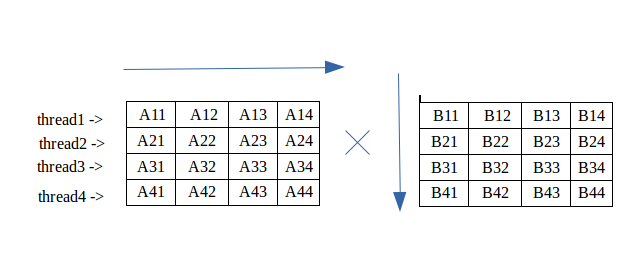
\includegraphics[width=3in]{matmul.png} 

\caption{Matrix multiplication using Pthreads \cite{pthreadwebsite}}
\label{pthread}
\end{figure}


 \pagebreak

\section{Comparison Tests}

\begin{itemize}

\item For comparing convolution using different kinds of matrix multiplication algorithms, a simple code was made in \verb!imgOp.cpp! called \verb!conv_mult_pad!. This function takes in a \verb!mult! input. The following values of \verb!mult! calls the following multiplication algortihms.

\begin{enumerate}
\item Simple Multiplication
\item 
 MKL multiplication
\item OpenBLAS multiplication
\item Pthread implementation of multiplication
\end{enumerate}

\item Then 10 matrices each with size from the range of 10 to 1000 were created with steps of 5 using \verb!matgen.cpp!

\item Using \verb!evaluator.cpp!, 4 different kernel sizes \emph{(3x3, 5x5, 7x7, 9x9)} were run on all the matrices and the running time was observed. The \verb!mean! \& \verb!standard deviation! of the running times of the 10 matrices were calculated and their plots were obtained (in figure~\ref{plot})

\begin{figure}[h]
	\centering
	\begin{tabular}{c c}
		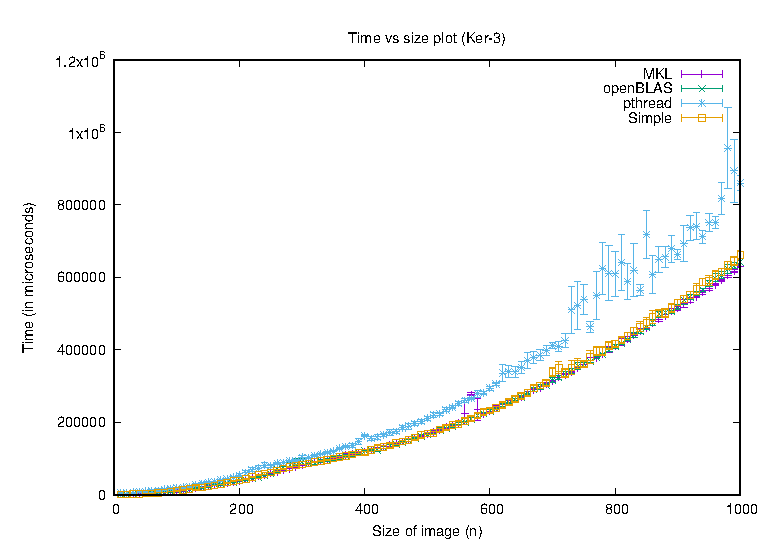
\includegraphics[width=3in]{plot_3.eps}  & 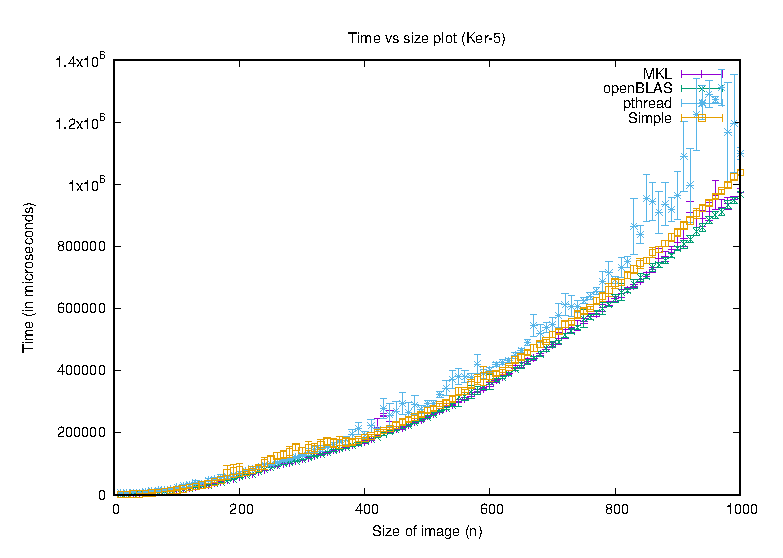
\includegraphics[width=3in]{plot_5.eps} \\ 
		 \small (a) Kernel = 3x3 & \small (b) Kernel = 5x5 \\
		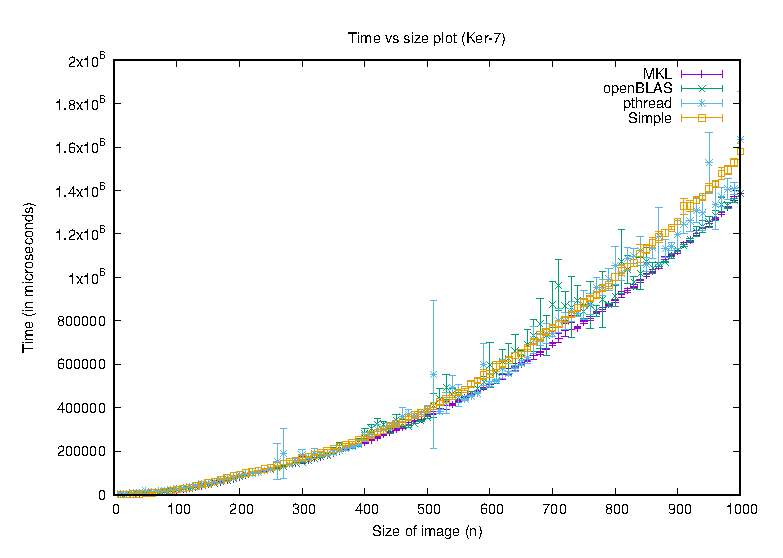
\includegraphics[width=3in]{plot_7.eps}  & 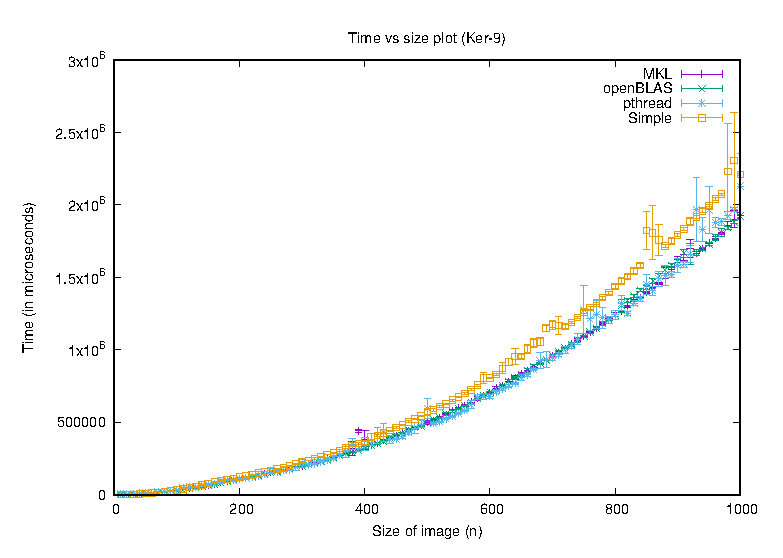
\includegraphics[width=3in]{plot_9.eps} \\ 
		 \small (c) Kernel = 7x7 & \small (d) Kernel = 9x9 \\
	\end{tabular}
	\caption{Time vs Size Plots}
	\label{plot}
\end{figure}

\item These results were run on an Intel i7 6th gen processor with 8 cores, and hence 8 threads were used.

\end{itemize}
\section{Observations}

\begin{itemize}
\item From the plots (figure~\ref{plot}), we can observe that the Intel MKL \cite{intelmkl} and OpenBLAS \cite{OpenBLAS} methods of matrix multiplication were the fastest for all the kernels with minimal error. All the plot seem to have O(\(n^3\)) nature. \emph{Note}: The optimised libraries are faster than O(\(n^3\)) algorithms.
\item  We can also notice that the pthread implementation reaches close to the faster implementations (calling the linear algebra libraries) when the kernel sizes are bigger. However, initially  it is even slower than simple multiplication for smaller kernels due to large overheads of creating pthreads.
\item However, it's clear that all these implementations are much faster than simple matrix multiplication for larger matrices. Only for fig~\ref{plot} (a), speed of simple multiplication almost matches that of the optimised libraries.
\item We also observe variations in times of the pthread implementation which may be due to memory issues/other processes already running in the cpu of the computer where the experiment was conducted.
\end{itemize}

\section{Conclusion}
The running times of many image processing libraries and functions such as convolution depend majorly on large scale matrix multiplication. This can be made much faster by using an optimized library such as Intel MKL \cite{intelmkl} or openBLAS \cite{OpenBLAS} can be speeded up using the multithreading concept. A combination of both can also be utilized which can speed up the running times of upcoming techniques like CNN's and applications of Computer Vision drastically to provide us with efficient and faster results.


% Generate the bibliography.
\bibliography{report}
\bibliographystyle{ieeetr}

\end{document}
